\section{Lazy Training in NNPDF (NOT FINAL)}
\label{sec:LazyTraining}

\begin{center}
  \red{Comments}\\
  \textcolor{blue}{Might be worth citing these two works for the NTH
  \cite{huang2019ddnn}\cite{Dyer:2019uzd}?}
\end{center}

\noindent In the previous section we presented an empirical study of the
training dynamics through the lens of the NTK. We observed that the NTK is able
to capture the main features of the training process, and that its time
evolution is characterised by a rapid initial transient, followed by a slower
evolution during the rest of the training. We now turn our attention on this
last stage of the training, where the NTK has stabilised and becomes
approximately constant. In doing so, we will build upon the results presented in
Refs.~\cite{jacot2018neural,lee2019wide} and extend them to the case of NNPDF.
In the following, we derive the analytical solution of the flow equation, which
allows us to write an explicit expression for the trained field as a function of
the field at initialisation and the data. We will discuss the phenomenological
implications of these results in Sec.~\ref{sec:TrainClosure}.

\subsection{Solution to the Flow Equation}
\label{sec:Lazy}

The lazy training regime is characterised by a slow-evolving NTK. We denote as
$T_{\rm ref}$ the time at which the onset of this regime occurs. The NTK is then
\textit{frozen} to its value at $T_{\rm ref}$, and from this time onward the NTK
is taken to be constant
\begin{equation}
  \Theta_t = \Theta_{T_{\rm ref}} \equiv \Theta, \quad \textrm{for } t \geq T_{\rm ref}.
\end{equation} 
The flow equation can then be written as
\begin{align}
  \ddt f_t = -\Theta M f_t + b\, ,
  \label{eq:FlowEqTwo}
\end{align}
where $M$ and $b$ are defined as in Eq.~\eqref{eq:MandBDef}. Note that now where
now neither $\Theta$ nor $b$ depend on the training time $t$, as a consequence
of the NTK. In order to solve this first-order linear differential equation, we
observe that the eigenvectors of $\Theta$,
\begin{align}
    \label{eq:ThetaEigensystem}
    \Theta z^{(k)} = \lambda^{(k)} z^{(k)}\, ,
\end{align}
provide a basis for expanding Eq.~\eqref{eq:FlowEqTwo}. It is necessary at this
stage to distinguish the components of $f_t$ that are in the kernel of $\Theta$
from the ones that are in the orthogonal complement, hence we introduce the
notation
\begin{align}
    \label{eq:ParallelCompnents}
    &f^\parallel_{t,k} = \left(z^{(k)}, f_t\right)\, , \quad \text{if}\ \lambda^{(k)} = 0\, , \\
    \label{eq:OrthogonalComponents}
    &f^\perp_{t,k} = \frac{1}{\sqrt{\lambda^{(k)}}} \left(z^{(k)}, f_t\right)\, , \quad
        \text{if}\ \lambda^{(k)} \neq 0\, ,
\end{align}
where the scalar product has been defined as
\begin{equation}
  \left(f'_{t'}, f_t\right) = \sum_{i,\alpha} f'_{t',i\alpha} f_{t,i\alpha}\,.
\end{equation}
One can readily see that the components in the kernel of $\Theta$, $\text{ker}\
\Theta$, do not evolve during the flow,\footnote{ Despite this result has been
obtained using the frozen NTK, it is worth mentioning that at any time during
training the kernel of the NTK is always defined and non-empty. Hence, also in
the initial stage, there will be a component that is completely determined by
the initial condition, \ie by the prior distribution in functional space.
\ac{This footnote might be expanded in the pheno section of NTK...}}
\begin{align}
    \label{eq:FlowParallel}
    \ddt f^\parallel_{t,k} = 0
        \quad \Longrightarrow \quad f^\parallel_{t,k} = f^\parallel_{0,k}\, .
\end{align}
This means that the final solution will be affected by an irreducible noise that
is purely dictated by the initial condition. The flow equation for the
orthogonal components can be written as
\begin{align}
    \label{eq:FlowPerp}
    \ddt f^\perp_{t,k} = - H^\perp_{kk'} f^\perp_{t,k'}
        + B^\perp_{k}\, ,
\end{align}
where  we introduced
\begin{align}
    H^\perp_{kk'} &= \sqrt{\lambda^{(k)}} \left(z^{(k)}, M z^{(k')}\right) \sqrt{\lambda^{(k')}}\, ,\\
    B^\perp_k &= -\sqrt{\lambda^{(k)}} \left[\left(z^{(k)}, M z^{(k')}\right) f^\parallel_{0,k'}
        - \left(z^{(k)}, \FKtabT C_Y^{-1} Y\right)\right]\, .
\end{align}
Here the indices on quantities that have a $\perp$ suffix only span the space
orthogonal to the kernel of $\Theta$, while the indices on quantities that have
a $\parallel$ suffix span the kernel. We refer to $H^\perp$ as the flow (or
training) Hamiltonian; we see explicitly in the definition above that the flow
dynamics is determined by a combination of the architecture of the NN, encoded
in the NTK, and the data, on which $M$ depends. More specifically, the matrix
elements of $M$ can be written as
\begin{align}
    \label{eq:MMatElems}
    \left(z^{(k)}, M z^{(k')}\right) = T^{(k)T} C_Y^{-1} T^{(k')}\, ,
\end{align}
where $T^{(k)} = T[z^{(k)}]$ is the vector of theory predictions for the data
obtained using $z^{(k)}$ as the input PDF. Similarly, we have
\begin{align}
    \label{eq:BMatElems}
    \left(z^{(k)}, \FKtabT C_Y^{-1} Y\right) = T^{(k)T} C_Y^{-1} Y\, .
\end{align}
Denoting by $d^\perp$ the dimension of the subspace orthogonal to $\text{ker}\
\Theta$, $H^\perp$ is a $d^\perp\times d^\perp$ symmetric matrix, whose
eigenvalues and eigenvectors satisfy
\begin{align}
    H^\perp_{kk'} w^{(i)}_{k'} = h^{(i)} w^{(i)}_{k}\, .
\end{align}
The solution to Eq.~\eqref{eq:FlowPerp} can be written as the sum of the
solution of the homogeneous equation, $\hat{f}^{\perp}_{t,k}$, and a particular
solution of the full equation. The solution of the homogeneous equation is
\begin{align}
    \label{eq:HomoSoln}
    \hat{f}^{\perp}_{t,k} = \sum_{i=1}^{d^\perp} f^{\perp}_{0,i} e^{-h^{(i)}t} w^{(i)}_k\, ,
\end{align}
where
% ~\footnote{ Note that here the scalar product is computed in the subspace
%     orthogonal to the kernel of $\Theta$,
%     \[
%         \left(w^{(i)}, f^\perp_0\right) = \sum_{k=1}^{d_\perp} w^{(i)}_{k} f^\perp_{0,k}
%     \]
% }
\begin{align}
    \label{eq:InitialCi}
    f^{\perp}_{0,i} = \sum_{k=1}^{d_\perp} w^{(i)}_k f^\perp_{0,k}\, ,
        %= \left(w^{(i)}, f^\perp_0\right)\, ,
\end{align}
guarantees that the initial condition $\hat{f}^\perp_{t,k}=f^\perp_{0,k}$ is
satisfied. Similarly, if we define
\begin{align}
    \label{eq:BiDef}
    \Upsilon^{(i)} = \sum_{k=1}^{d_\perp} w^{(i)}_k B^\perp_{k}\, ,
        %= \left(w^{(i)}, B^\perp\right)\, ,
\end{align}
then
\begin{align}
    \label{eq:PartSol}
    \check{f}^\perp_{t,k} = \sideset{}{'}\sum_{i} \frac{1}{h^{(i)}} \Upsilon^{(i)}
        \left(1 - e^{-h^{(i)}t}\right) w^{(i)}_k\, ,
\end{align}
where the sum only involves the non-zero modes of $H^\perp$, is a particular
solution of the inhomogeneous equation, which satisfies the boundary condition
$\check{f}^{\perp}_{0,k}=0$. Finally, the solution of the flow equation in the
subspace orthogonal to $\text{ker}\ \Theta$ is
\begin{align}
    f^\perp_{t,k}
    \label{eq:FlowSolution}
        &= \hat{f}^\perp_{t,k} + \check{f}^\perp_{t,k}
        % &= \sum_{i=1}^{d^\perp}  \left(w^{(i)}, f^\perp_0\right) e^{-h^{(i)}t} w^{(i)}_k
        %     + \sideset{}{'}\sum_{i=1}  \frac{1}{h^{(i)}} \left(w^{(i)}, B^\perp\right)
        %         \left(1 - e^{-h^{(i)}t}\right) w^{(i)}_k
        \, .
\end{align}
Finally, collecting the parallel contribution, Eq.~\eqref{eq:FlowParallel}, and
the solution of the orthogonal component, Eq.~\eqref{eq:FlowSolution}, yields a
simple expression,
\begin{align}
    \label{eq:AnalyticSol}
    f_{t,\alpha}
        = U(t)_{\alpha\alpha'} f_{0,\alpha'} + V(t)_{\alpha I} Y_{I}\, .
\end{align}
The two evolution operators $U(t)$ and $V(t)$ have lengthy, yet explicit,
expressions, which we summarise here: 
\begin{align}
    U(t)_{\alpha\alpha'} = \hat{U}^\perp(t)_{\alpha\alpha'}
        + \check{U}^\perp(t)_{\alpha\alpha'} + U^\parallel_{\alpha\alpha'}\, ,
\end{align}
where
\begin{align}
    \hat{U}^\perp(t)_{\alpha\alpha'}
        = \sum_{k,k'\in\perp} \sqrt{\lambda^{(k)}} z^{(k)}_\alpha 
            \left[\sum_i w^{(i)}_{k} e^{-h^{(i)}t} w^{(i)}_{k'}\right]
            z^{(k')}_{\alpha'} \frac{1}{\sqrt{\lambda^{(k')}}}\, ,
\end{align}
and
\begin{align}
    U^\parallel_{\alpha\alpha'}
        = \sum_{k''\in\parallel} z^{(k)}_\alpha z^{(k)}_{\alpha'} \, .
\end{align}
The contributions from $\check{U}^\perp(t)$ and $V(t)$ are more easily expressed
by introducing the operator
\begin{align}
    \label{eq:MOperatorDef}
    \mathcal{M}(t)_{\alpha\alpha'} 
        = \sum_{k,k'\in\perp} \sqrt{\lambda^{(k)}} z^{(k)}_\alpha 
            \left[\sideset{}{'}\sum_{i} w^{(i)}_{k} \frac{1}{h^{(i)}}\, 
            \left( 1- e^{-h^{(i)}t}\right) w^{(i)}_{k'}\right]
            z^{(k')}_{\alpha'} \sqrt{\lambda^{(k')}}\,. 
\end{align}
Then, we can write
\begin{align}
    \label{eq:UperpCheck}
    \check{U}^\perp(t)
        = - \mathcal{M}(t)\; \FKtabT C_Y^{-1} \FKtab 
            \left[\sum_{k''\in\parallel} z^{(k'')} z^{(k'') T}\right]\, ,
\end{align}
and
\begin{align}
    V(t) = \mathcal{M}(t)\; \FKtabT C_Y^{-1}\, ,
\end{align}
where we note that the term in the bracket in Eq.~\eqref{eq:UperpCheck} is
simply the projector on the kernel of the NTK. The four terms that appear in the
analytical solution have a clear physical interpretation:
\begin{itemize}
    \item The first term $\hat{U}^\perp(t)$ suppresses the components of the
    initial condition that lie in the subspace orthogonal to the kernel of the
    NTK. These are the components that are learned by the network during
    training. While the trained solution still depends on its value at
    initialisation, that dependence is suppressed during training. This
    suppression is exponential in the training time, and the rates are given by
    the eigenvalues of $H^{\perp}$.
    \item The contribution from $U^\parallel$ yields the component of the
    initial condition that lies in the kernel of the NTK. As such, those
    components remain unchanged during training and are part of the trained
    field at all times $t$. 
    \item The two remaining contributions are best understood by combining them
    together,
    \begin{align}
        \label{eq:DataCorrectedInference}
        \check{U}^{\perp}(t) f_{0} + V(t) Y 
            = \mathcal{M}(t)\; \FKtabT C_Y^{-1} \left[Y - \FKtab f_{0}^{\parallel}\right]\, .
    \end{align}
    The parallel component of the initial condition $f_{0}^{\parallel}$ does not
    evolve during training, and therefore it yields a contribution $\FKtab
    f_{0}^{\parallel}$ to the theoretical prediction of the data points at all
    times $t$. This is taken into account by subtracting this contribution from
    the data, before the inference is performed.
\end{itemize}
The solution in Eq.~\eqref{eq:AnalyticSol} is the main result of this section.
It shows that the training process can be described as the sum of a linear
transformation of the initial fields $f_{0,\alpha}$, which are the
preactivations of the output layer at initialisation, and a linear
transformation of the data $Y_I$. The two transformations depend on the flow
time $t$ and are given by the evolution operators $U(t)$ and $V(t)$.
Eq.~\eqref{eq:AnalyticSol} encodes the information on the central value and the
variance of the trained fields, and any other quantity that is derived from the
PDFs.

Before moving on, a clarification is in order. We have been using the term
``initial condition'' without specifying what it exactly means in this context.
Indeed, the initial condition can be taken to be the value of the trained
network at the $T_{\rm ref}$, \ie the time at which we pick the NTK. In this
case Eq.~\eqref{eq:AnalyticSol} would provide the continuation of the training
from $T_{\rm ref}$ onward, provided we are in the lazy regime. However, the
initial condition can also be sample from a prior distribution, for instance it
could be a replica of the network ensemble at initialisation.

\subsubsection{Central value and Covariance of the trained fields}
\label{sec:CentralAndCovariance}

\noindent In deriving the analytical solution in Eq.~\eqref{eq:AnalyticSol}, we
implicitly considered a single realization of the frozen NTK over the ensemble.
However, we are interested in the analytical evolution of the ensemble of
trained networks, which can be obtained by considering the different replicas of
the frozen NTK. Thus, the operators $U(t)$ and $V(t)$ that enter
Eq.~\eqref{eq:AnalyticSol} should be considered as random variables distributed
according to the ensemble. Moreover, the initial condition $f_0$ is also a
random variable, while the data fluctuations in the data $Y$ depend on
how the artificial data replicas are constructed.

As a consequence, the analytical solution in Eq.~\eqref{eq:AnalyticSol} becomes
a random variable. We can then characterize its distribution using the mean and
variance across the ensemble of analytical solutions, as shown in
Eq.~\eqref{eq:ReplicaEnsemble}. The central value of the trained field is thus
defined as
\begin{align}
    \label{eq:MeanValAtT}
    \bar{f}_{t,\alpha} = \mathbb{E}\left[f_{t,\alpha}\right]
        = \mathbb{E}\left[U(t)_{\alpha\alpha'} f_{0,\alpha'}\right]
            + \mathbb{E}\left[V(t)_{\alpha I} Y_I\right] \, .
\end{align}
Note that the first term on the right-hand side of Eq.~\eqref{eq:MeanValAtT} can
only be non-zero because of the correlations between $U(t)$ and $f_0$. In the
absence of such correlations, the first term would be given by the product of
the expectation values. In $f_0$ is an ensemble of networks at initialisation,
the we now from the theory in Sec.~\ref{sec:Init} that the expectation value
of the output vanishes.

and hence would vanish up to corrections of order
$\mathcal{O}(1/n)$, since the expectation value of the fields at initialisation
vanishes in the limit of infinitely wide networks. Assuming that the
correlations between the initial fields and the evolution operators vanish, we
can write
\begin{align}
    \label{eq:MeanUt}
    \bar{U}(t)
        &= \mathbb{E}\left[U(t)\right]\, , \\
    \label{eq:MeanVt}
    \bar{V}(t)
        &= \mathbb{E}\left[V(t)\right]\, ,
\end{align}
and
\begin{equation}
    \label{eq:MeanValAtTNoCorr}
    \bar{f}_{t,\alpha} = \bar{U}(t)_{\alpha\alpha'} \bar{f}_{0,\alpha'}
        + \bar{V}(t)_{\alpha I} Y_I = \bar{V}(t)_{\alpha I} Y_I \, .
\end{equation}
The second term in Eq.~\eqref{eq:MeanValAtT}, or equivalently
Eq.~\eqref{eq:MeanValAtTNoCorr}, explicitly shows the contribution of each data
point to the central value of the trained fields at each value of $x_{\alpha}$.
It is worthwhile remarking that in this limit, the central value from the set of
trained networks is a linear combination of the data points, with coefficients
given by the evolution operator $V(t)_{\alpha I}$. It is worth mentioning that
Eq.~\eqref{eq:FlowSolution} resembles the structure of a linear method,
like \eg\ Backus-Gilbert or Gaussian Processes. We will comment further on this
point later in this section.

For the covariance we have 
\begin{align}
    \cov[f_t,f_t^T]
        &= \mathbb{E}\left[U(t) f_0 f_0^T U(t)^T\right] 
            - \mathbb{E}\left[U(t) f_0\right] \mathbb{E}\left[f_0^T U(t)^T\right]  \nonumber \\
        &\quad + \mathbb{E}\left[U(t) f_0 Y^T V(t)^T\right] 
            - \mathbb{E}\left[U(t) f_0\right] \mathbb{E}\left[Y^T V(t)^T\right] \nonumber \\
        &\quad + \mathbb{E}\left[V(t) Y f_0^T U(t)^T\right]
            - \mathbb{E}\left[V(t) Y\right] \mathbb{E}\left[f_0^T U(t)^T\right] \nonumber \\
    \label{eq:CovAtT}
        &\quad + \mathbb{E}\left[V(t) Y Y^T V(t)^T\right]
            - \mathbb{E}\left[V(t) Y\right] \mathbb{E}\left[Y^T V(t)^T\right] \, .
\end{align}
Note that the first and the fourth lines above yield symmetric matrices, while
the third line is just the transpose of the second, thereby ensuring that the
whole covariance matrix is the sum of three symmetric matrices and therefore is
symmetric, 
\begin{align}
    \label{eq:SumOfCovariances}
    \cov[f_t,f_t^T] = C_t^{(00)} + C_t^{(0Y)} + C_t^{(YY)}\, ,
\end{align}
where
\begin{align}
    \label{eq:C00term}
    C_t^{(00)} 
        &= \mathbb{E}\left[U(t) f_0 f_0^T U(t)^T\right] 
        - \mathbb{E}\left[U(t) f_0\right] \mathbb{E}\left[f_0^T U(t)^T\right]\, ,\\
    C_t^{(0Y)}
        &= \mathbb{E}\left[U(t) f_0 Y^T V(t)^T\right] 
        - \mathbb{E}\left[U(t) f_0\right] \mathbb{E}\left[Y^T V(t)^T\right] \nonumber \\
        \label{eq:C0Yterm}
        &\quad + \mathbb{E}\left[V(t) Y f_0^T U(t)^T\right]
            - \mathbb{E}\left[V(t) Y\right] \mathbb{E}\left[f_0^T U(t)^T\right] \, ,\\
    C_t^{(YY)}
        &= \mathbb{E}\left[V(t) Y Y^T V(t)^T\right]
        - \mathbb{E}\left[V(t) Y\right] \mathbb{E}\left[Y^T V(t)^T\right]\, .
\end{align}

% Onset Lazy L0 ===================================
\begin{figure}[t]
  \centering
  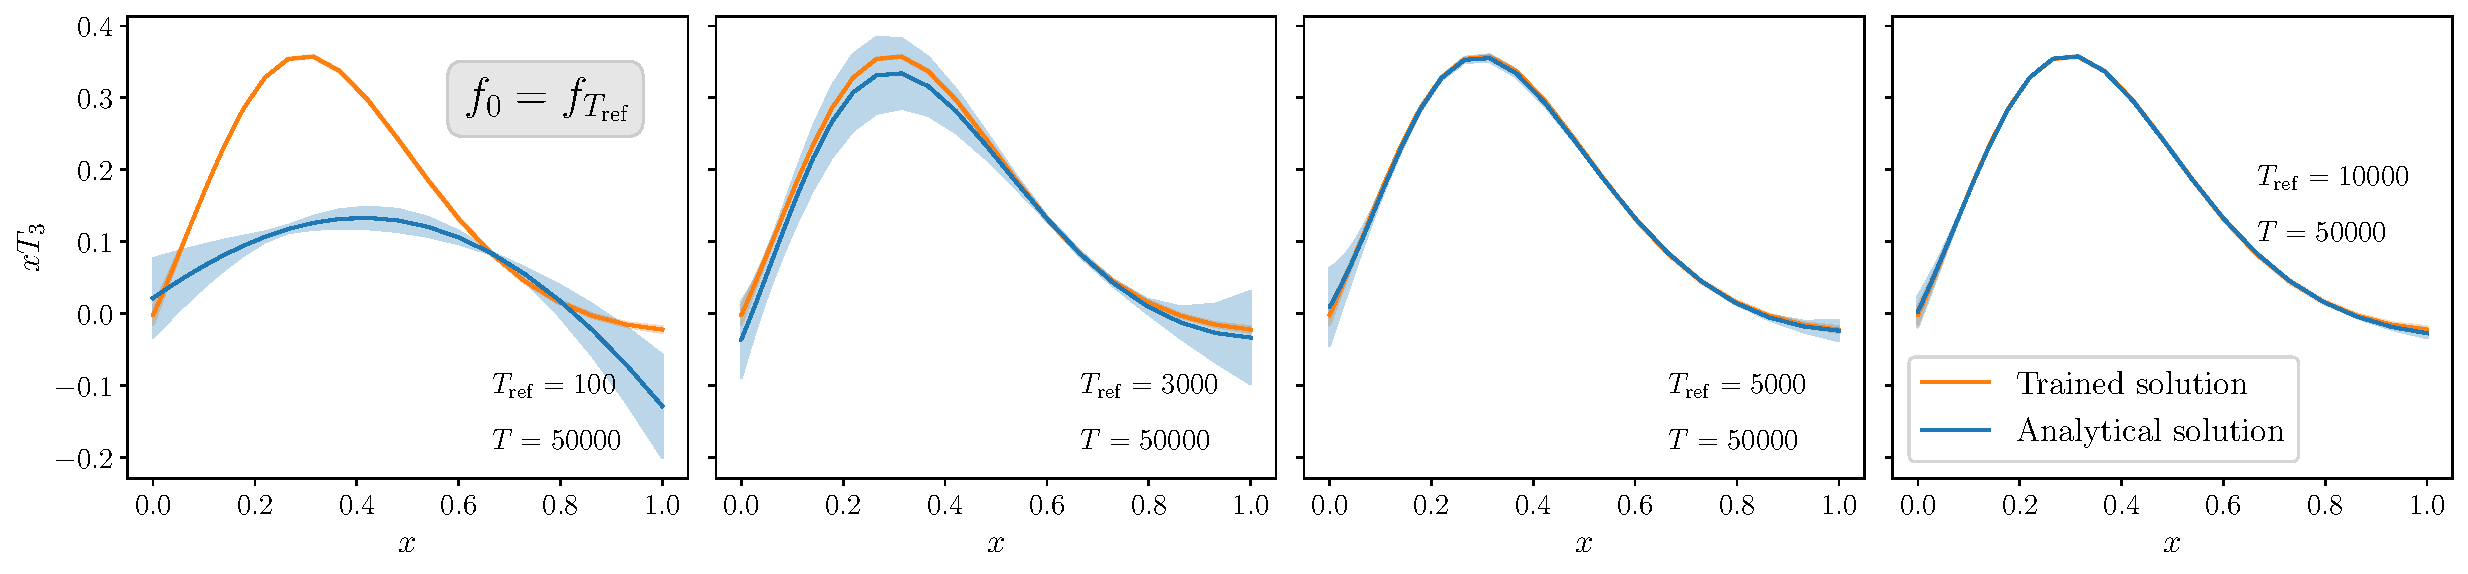
\includegraphics[width=0.9\textwidth]{section_4/evolution_vs_trained_ftref_L0.pdf}
  \caption{Comparison of the trained and analytical evolution at the end of
  training. In each panel, the blue curve remains identical. The analytic
  evolution is obtained using the NTK frozen at $T_{\rm ref}$, which is
  different in each panel. The initial condition is taken from the ensemble at
  $T_{\rm ref}$, then evolved analytically until the end of training}
  \label{fig:OnsetLazyL0}
\end{figure}
% =================================================
% Onset Lazy L1 ===================================
\begin{figure}[t]
  \centering
  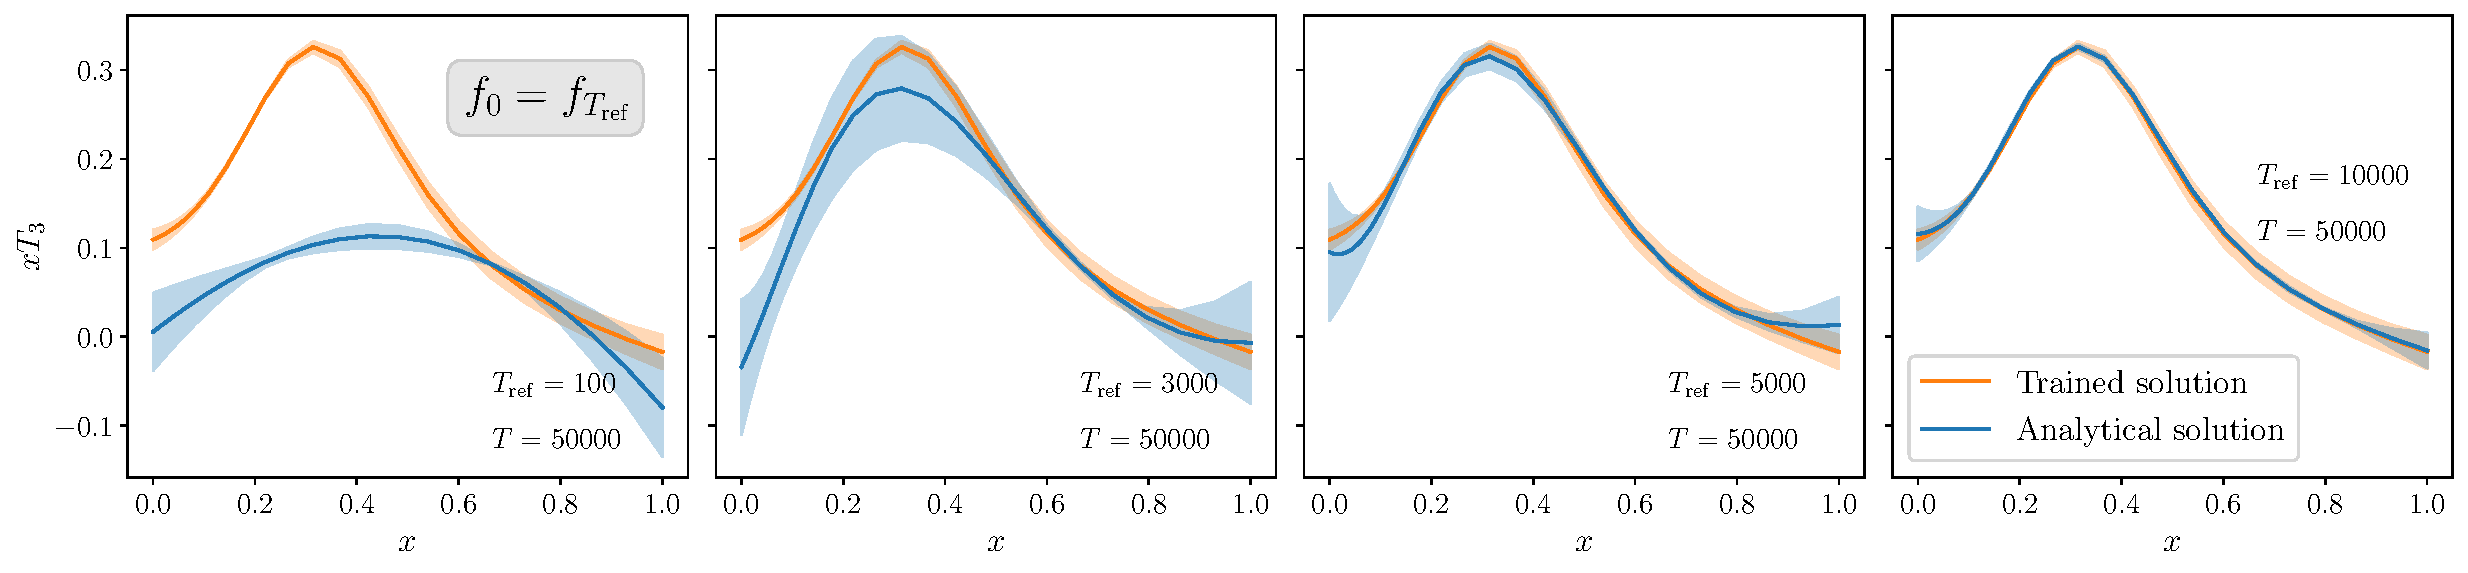
\includegraphics[width=0.9\textwidth]{section_4/evolution_vs_trained_ftref_L1.pdf} 
  \caption{Same as Fig.~\ref{fig:OnsetLazyL0}, but for L1 closure test data.}
  \label{fig:OnsetLazyL1}
\end{figure}
% =================================================
% Onset Lazy L2 ===================================
\begin{figure}[t]
  \centering
  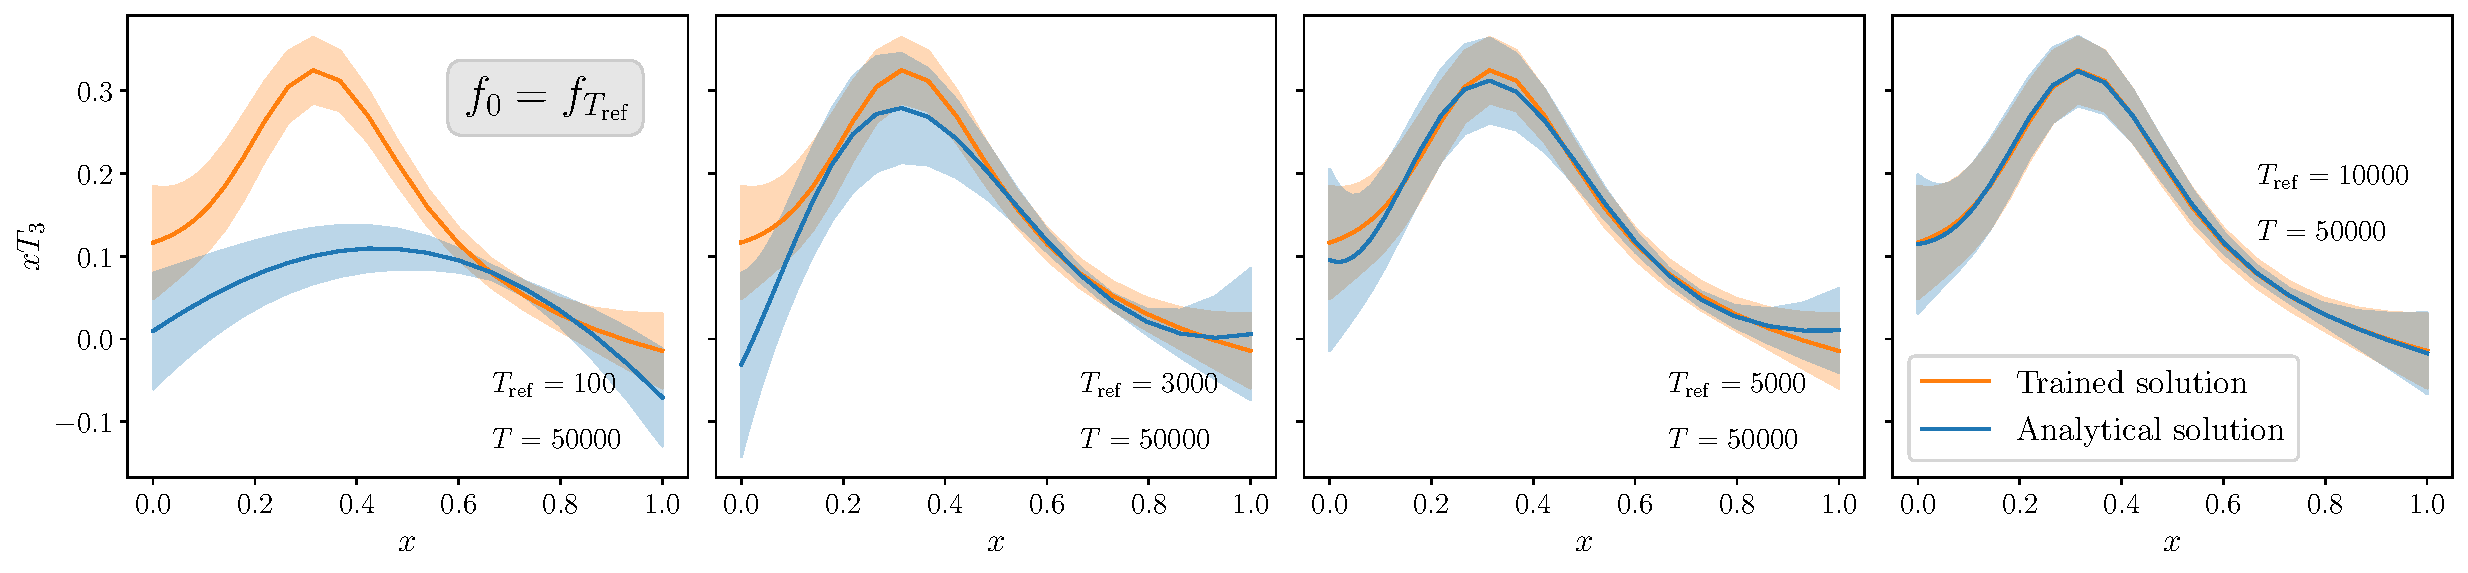
\includegraphics[width=0.9\textwidth]{section_4/evolution_vs_trained_ftref_L2.pdf} 
  \caption{Same as Fig.~\ref{fig:OnsetLazyL0}, but for L2 closure test data.}
  \label{fig:OnsetLazyL2}
\end{figure}
% =================================================

% Decomposition L0 ================================
\begin{figure}[t]
  \centering
  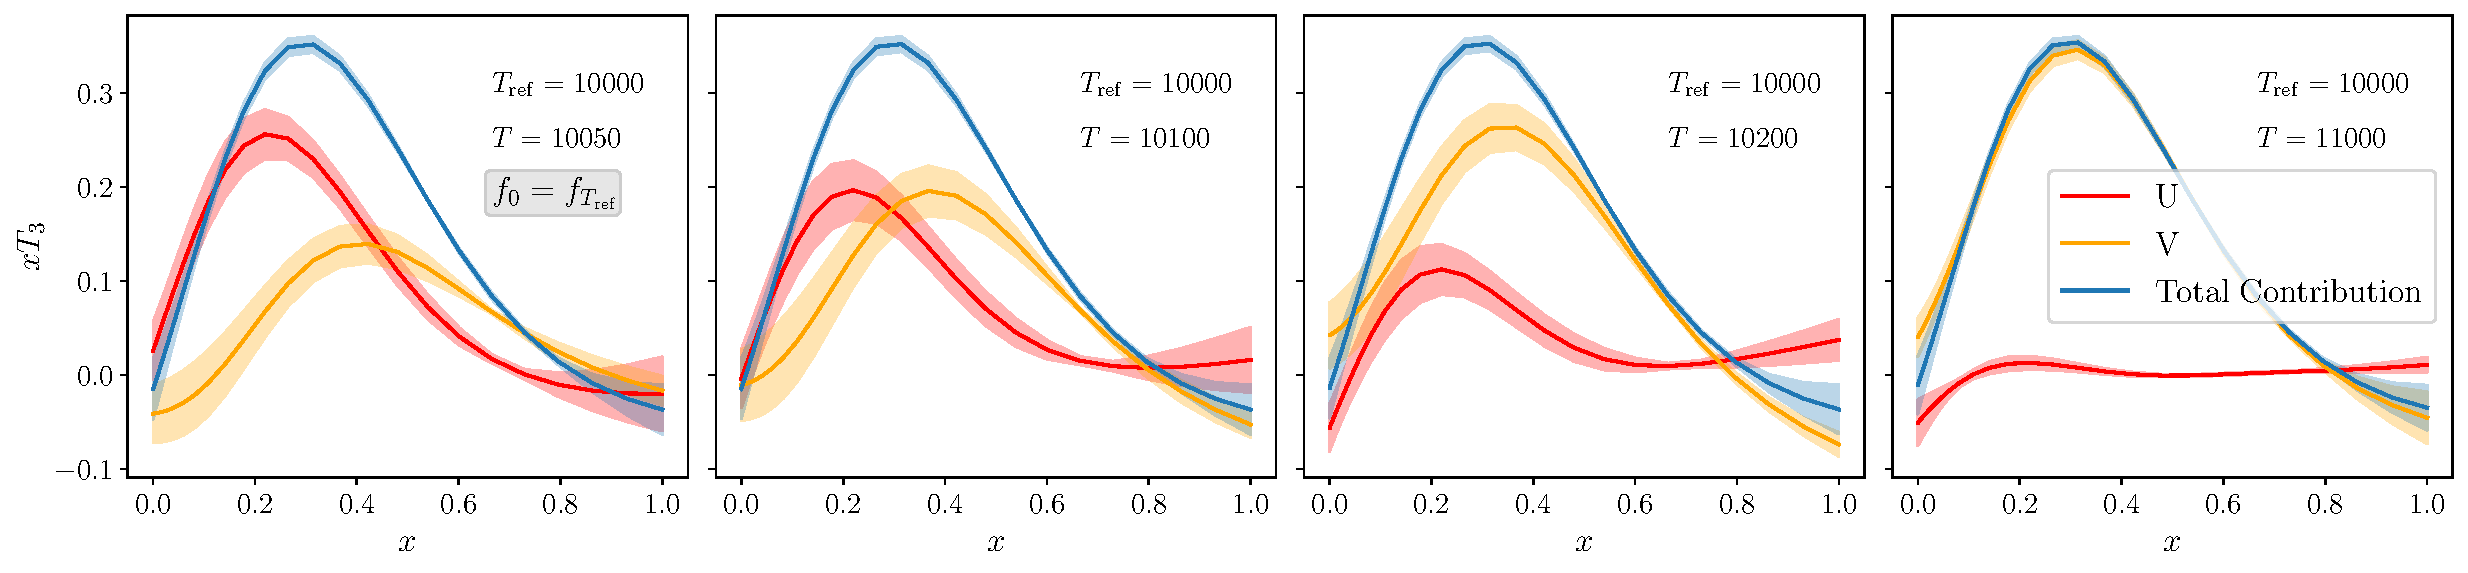
\includegraphics[width=0.9\textwidth]{section_4/u_v_decomposition_L0.pdf}
  \caption{Decomposition of the trained field into the $U$ and $V$ components
  at different training time with fixed frozen NTK at $T_{\rm ref}$. The initial
  condition is taken from the ensemble at $T_{\rm ref}$, then evolved
  analytically. L0 data is used.}
  \label{fig:FrefDecompositionL0}
\end{figure}
% =================================================
% Decomposition L1 ================================
\begin{figure}[t]
  \centering
  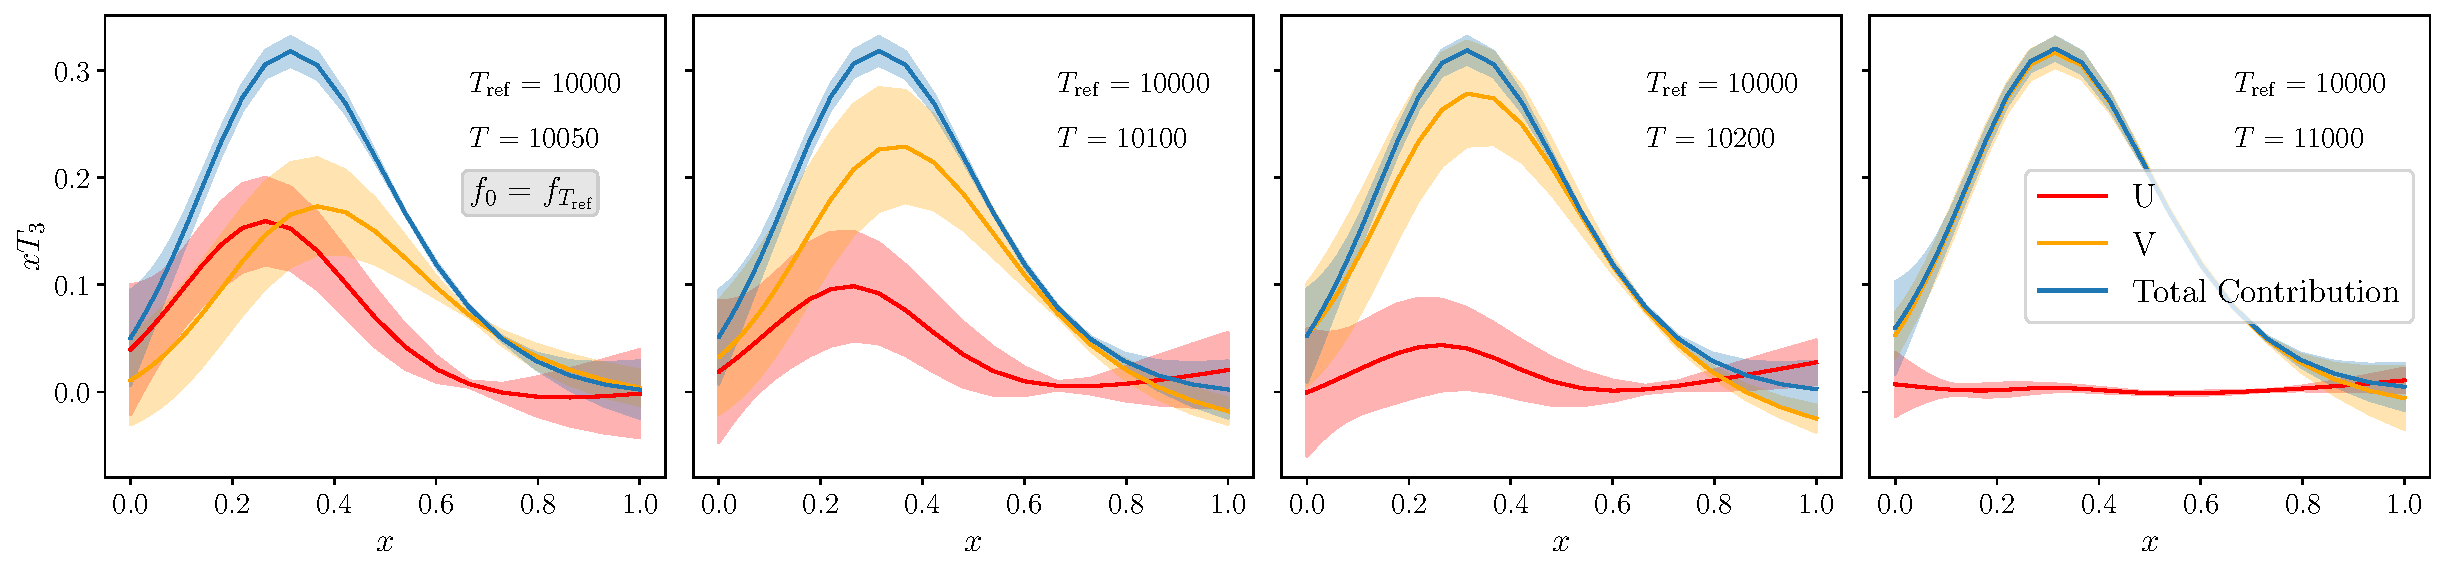
\includegraphics[width=0.9\textwidth]{section_4/u_v_decomposition_L1.pdf} 
  \caption{Same as Fig.~\ref{fig:FrefDecompositionL0}, but for L1 closure test
  data.}
  \label{fig:FrefDecompositionL1}
\end{figure}
% =================================================
% Decomposition L2 ================================
\begin{figure}[t]
  \centering
  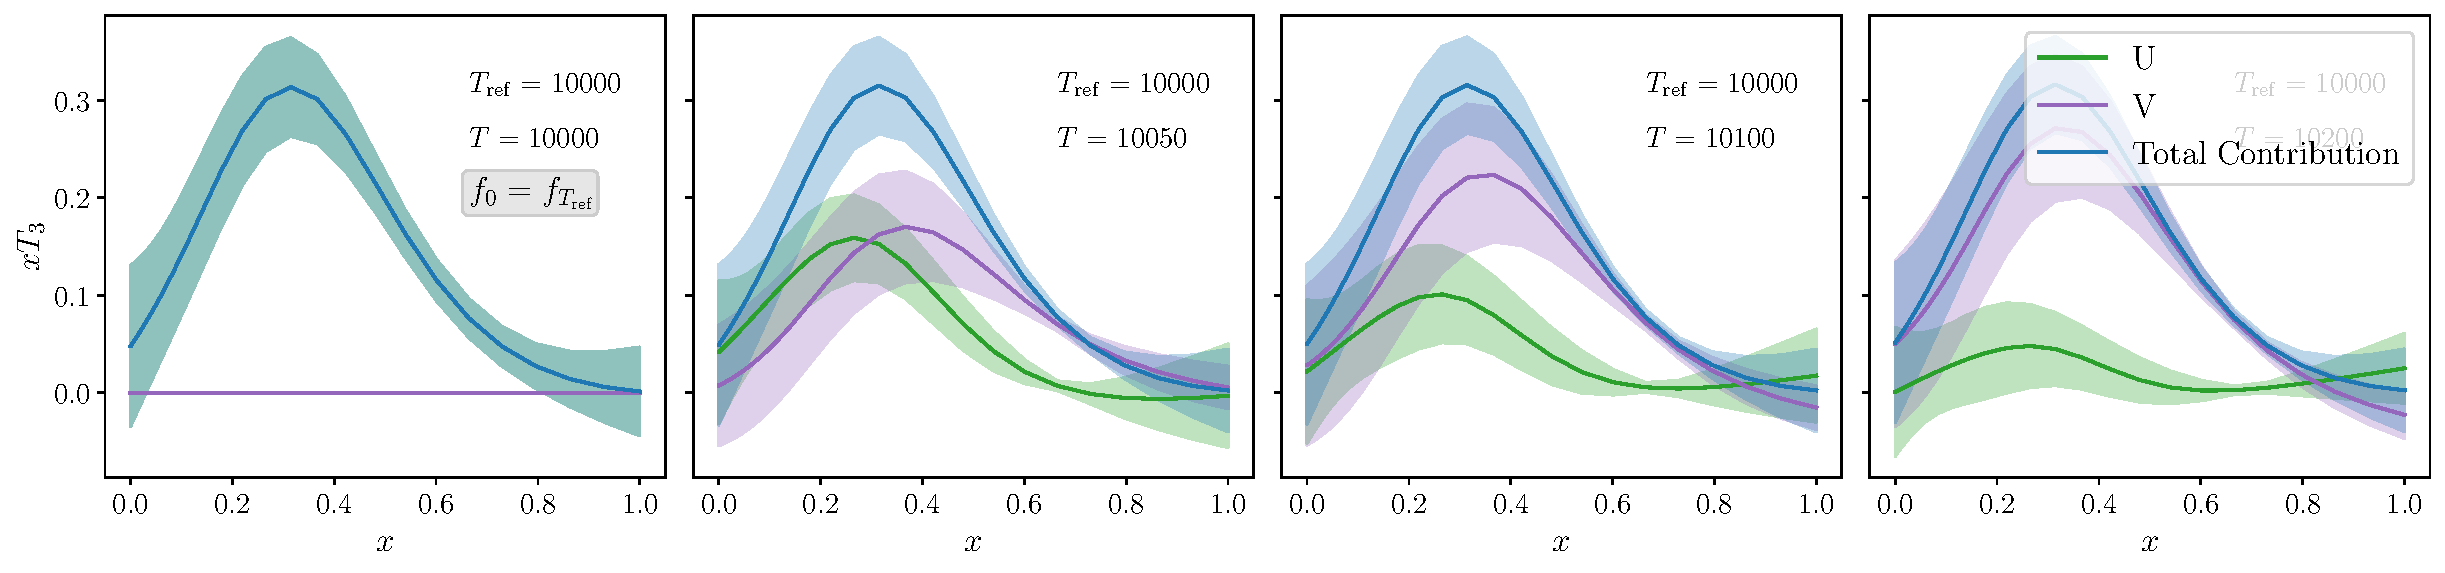
\includegraphics[width=0.9\textwidth]{section_4/u_v_decomposition_L2.pdf} 
  \caption{Same as Fig.~\ref{fig:FrefDecompositionL0}, but for L2 closure test
  data.}
  \label{fig:FrefDecompositionL2}
\end{figure}
% =================================================

\subsection{Results and Crosschecks}
\label{sec:TrainClosure}

The analytical solution in Eq.~\eqref{eq:AnalyticSol} sheds a new light onto the
behaviour of the numerical neural network training. In order to study the
training process, the NNPDF collaboration has successfully developed so-called
{\em closure tests}, which we are going to adopt here. 

A closure test uses synthetic data, generated using a known set of PDFs, to
train the neural network. The PDFs used for generating the data are called here
{\em input}\ PDFs. The results of the training are then compared to the known
input PDFs; the performance of the training algorithm and the NN architecture
are assessed by quantifying the comparison between trained PDFs and input PDFs.
Following the original presentation in Ref.~\cite{NNPDF:2014otw}, we distinguish
three levels of closure tests, which are defined by the complexity of the data
used to train the NNs. We use the standard NNPDF nomenclature and refer to these
three levels as level-0 (L0), level-1 (L1), and level-2 (L2) closure tests, and
we denote the input PDFs used to generate the data as $\fin$.

With the full control over the sought solution at hand, the analytic solution
allows us to perform a number of crosschecks that validate our implementation
and provides insight into the training process. These are discussed in the
following sections.

\subsection{Analytical Results and Crosschecks using L0 data}
\label{sec:AnalyticalChecks}
Let us start by discussing the case of L0 closure tests. In this case, the realization
of the dataset is completely determined by the input PDFs, and the values of the data
are given by
\begin{equation}
    \label{eq:DataL0}
    Y_I = T[\fin]_I
        = \sum_{i=1}^{\nflav} \sum_{\alpha=1}^{\ngrid} \FKtab_{Ii\alpha} \fin_{i\alpha}\, ,
\end{equation}
or equivalently, suppressing the indices,
\begin{equation}
    \label{eq:DataL0NoIndices}
    Y = \FKtab \fin\, .
\end{equation}
Note that using L0 data only affects the second term in
Eq.~\ref{eq:AnalyticSol}\footnote{To be more precise, since the analytical
solution is requires the NTK to be frozen at a certain epoch $T_{\rm ref}$, the
NTK will itself depend on the data used in the training.}. We can then rewrite the
combined term in Eq.~\eqref{eq:DataCorrectedInference} as follows
\begin{align}
  \label{eq:TrainingOnLevelZero}
  \check{U}^\perp(t) f_0 + V(t) Y 
    &= \mathcal{M}(t)\, \FKtabT C_{Y}^{-1} \FKtab\, 
      \left[\fin - f_{0}^\parallel\right]\, .
\end{align}
The subtraction taking place in the square brackets of
Eq.~\eqref{eq:TrainingOnLevelZero} suggests us that the effective function that
the neural network actually sees is not the input function $\fin$ used to
generate the data, but rather the difference between $\fin$ and the component of
the initial function $f_0$ that lies in the subspace spanned by the kernel of
the NTK, \ie\ $f_0^\parallel$. In other words, the parallel component
$f_0^\parallel$, which we remind does not evolve during the analytic training,
acts as a constant ``bias'' in the training process, shifting the effective
input function that the neural network sees. Of course the actual magnitude of
this irreducible noise depends both on how $f_0$ and the kernel of the NTK are
distributed over the ensemble. We will come to this point soon.

Note that the observation above remains true even in the limit of infinite training.
This can be shown using
Interestingly, for $t\to\infty$, we have
\begin{align}
    \label{eq:LevelZeroClosureInfiniteTraining}
    \lim_{t\to\infty} V(t) Y = \finperp + \mathcal{M}_{\infty} M \finpar
\end{align}
and therefore the $V$ component of the trained solution reproduces exactly the
component of the PDF that lies in  the subspace orthogonal to the kernel of
$\Theta$. We compare the asymptotic behaviour of $V(t) Y$ and $\finperp$ in
Fig.~\ref{fig:InfiniteTimeVterm}.

\begin{figure}[t]
  \centering
  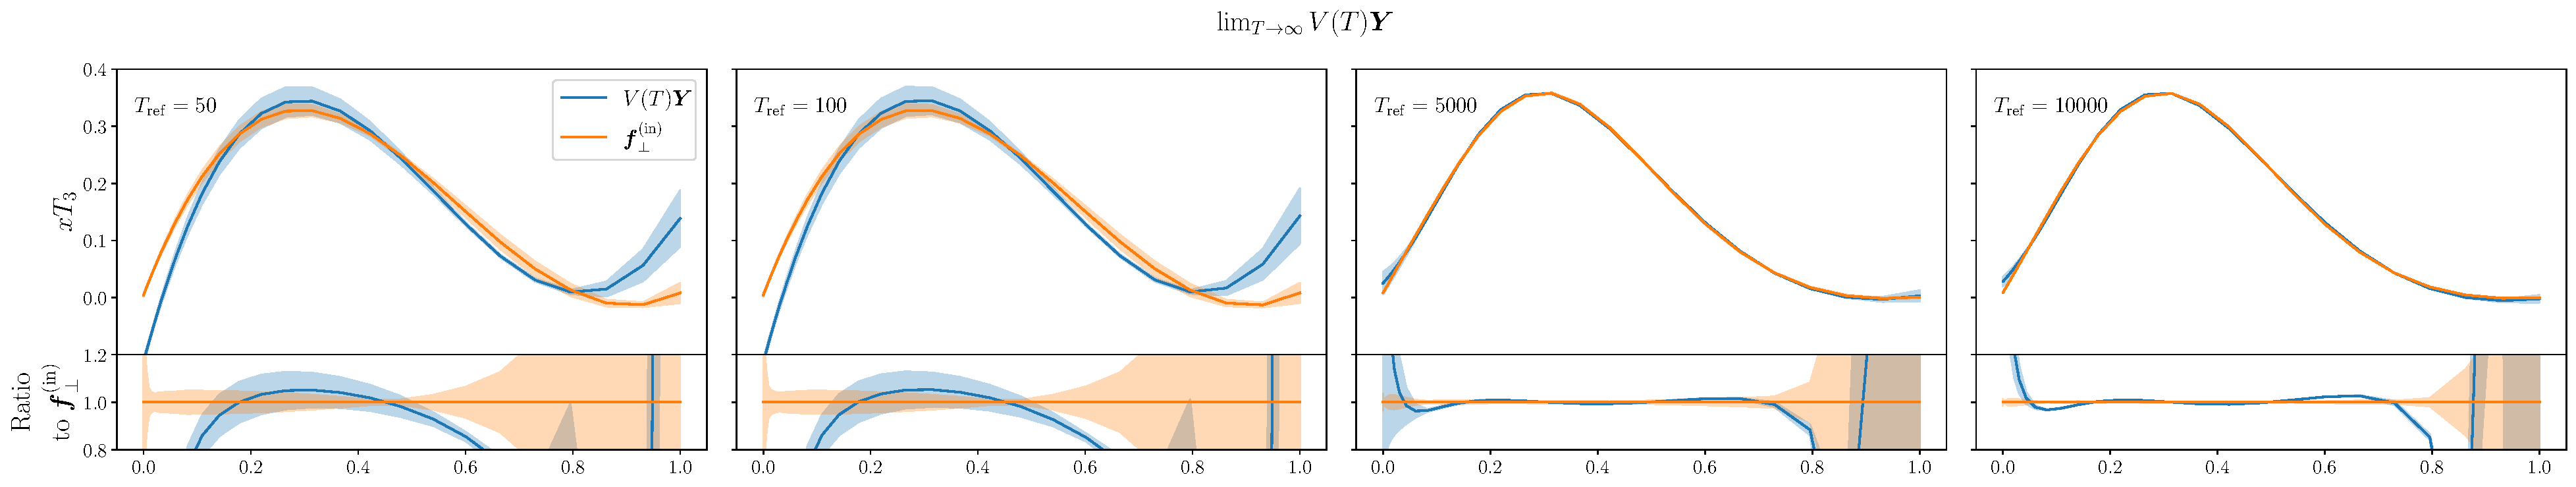
\includegraphics[width=\textwidth]{vy_inf_L0.pdf}  
  \caption{Test the $t\to\infty$ limit of the L0 training for different frozen
  NTK. The orange curve represents the projection of the input function $\fin$
  onto the subspace orthogonal to the kernel of the NTK at $T_{\rm ref}$, \ie\
  $\finperp$. The blue curve represents the contribution of the operator $V$,
  computed with the NTK at $T_{\rm ref}$, in the limit of infinite training
  time.}
  \label{fig:InfiniteTimeVterm}
\end{figure}

The second term in the square bracket on the right-hand side of
Eq.~\eqref{eq:TrainingOnLevelZero} is the contribution from the parallel
component at initialisation that does not evolve in the training process. Given
that $f_0$ is almost normally distributed around zero, that term does not
contribute to the central value of the fitted PDF, \ie\ to the average of the
trained solution over replicas. The time evolution of 
\begin{align}
  \label{eq:AverageLevelZeroUcheck}
  \mathbb{E}\left[\mathcal{M}(t)\, \FKtabT C_{Y}^{-1} \FKtab\, 
    f_{0}^\parallel\right]\, ,
\end{align}
is shown in Fig.~\ref{fig:AverageLevelZeroUcheck}.
\begin{figure}[h!]
  \centering
  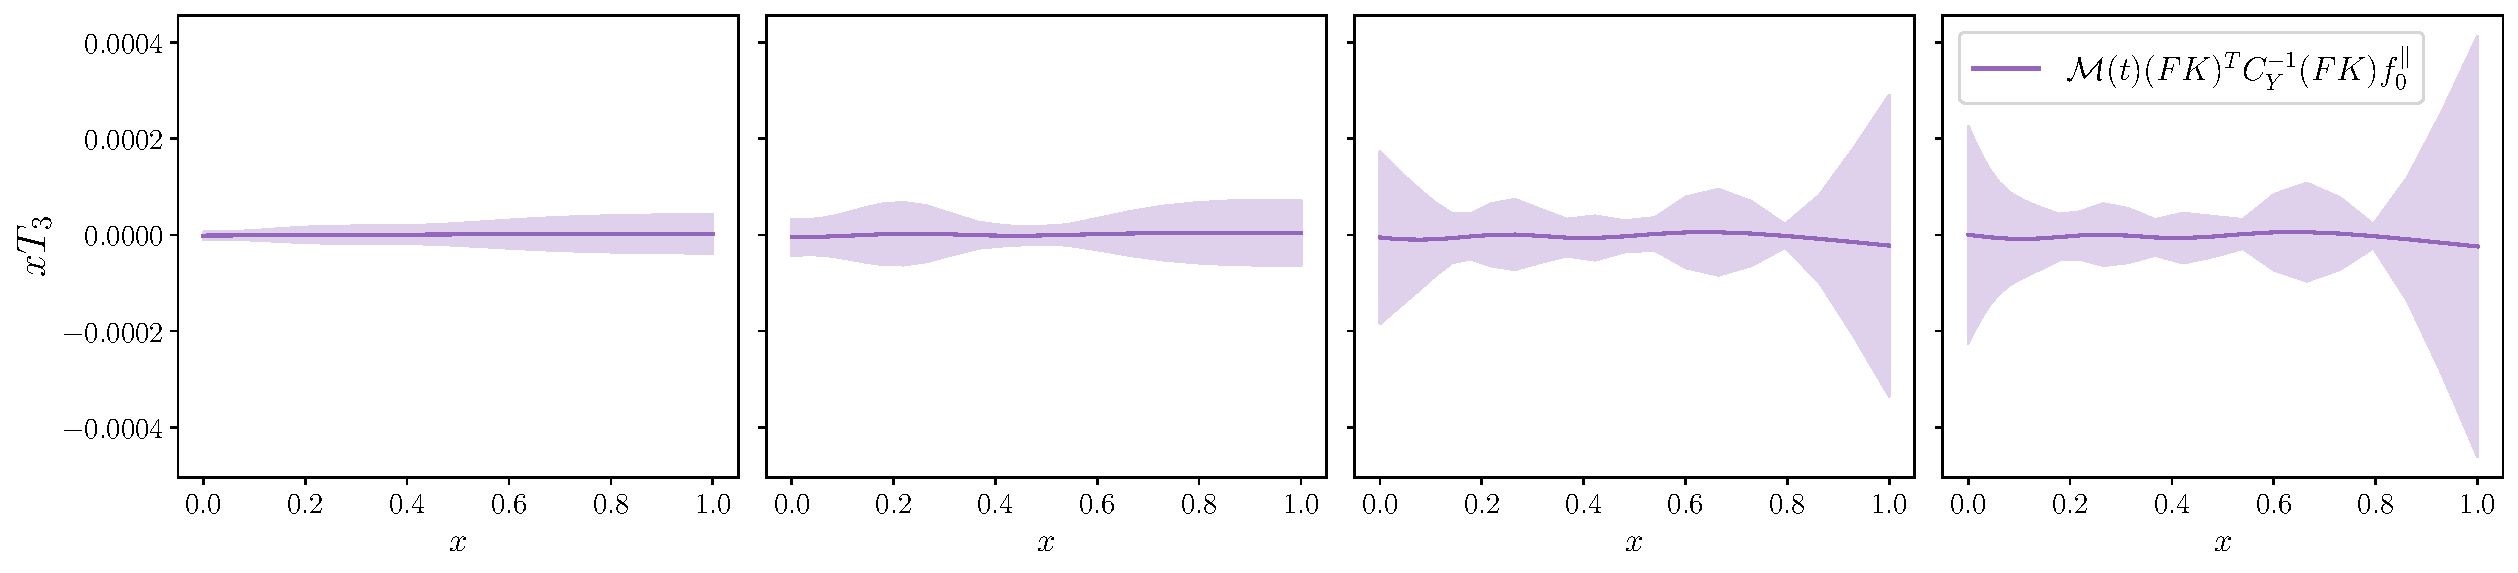
\includegraphics[width=0.95\textwidth]{Mcal_M_fpar_L2_linear.pdf} 
  \caption{Test of the average of the parallel contribution for different
  epochs. The reference epoch at which the frozen NTK is chosen is $T_{\rm ref}
  = 10000$. L2 data is used in the plot.}
  \label{fig:AverageLevelZeroUcheck}
\end{figure}

\FloatBarrier

\subsubsection{Convergence of the Analytical Solution}
\label{sec:CheckAnalyticalConvergence}

At the beginning of the training process there is clearly no difference between
the analytical solution and the trained solution. By construction both AS and TS
are given by the outcome of the neural network at initialisation, as discussed
in Sect.~\ref{sec:Init}. In the early stages of training AS and TS differ as
expected. Indeed, the analytical solution is computed using the frozen NTK at
$T_{\rm ref}$, while the trained solution evolves with an NTK that is still
changing as shown in Sect.~\ref{sec:NTKPheno}. Since the NTK at $T_{\rm ref}$ is
already aligned with the solution, the AS converges faster to the target
solution, while the TS takes more epochs before starting to evolve in the right
direction. The two solutions are compared for different training times in
Fig.~\ref{fig:xT3_analytical_vs_trained} after $T=500, 1000$ and 10000 epochs.
The plots in the left column correspond to synthetic L0 data, while the ones in
the right column are obtained using L2 data. The analytical solution is obtained
using a frozen NTK at $T_{\rm ref}=20000$. In both cases the analytical solution
agrees with the trained one for $T=10000$.

\begin{itemize}
  \item Trained vs Analytical solution at different training times (grid)
  \item Decomposition of U and V
  \item Error decomposition
\end{itemize}

\subsubsection{Error decomposition}

\subsubsection{Infinite Training Time}
In the limit of infinite training time, the evolution operators $U(t)$ and
$V(t)$ simplify and yield an elegant interpretation of the minimum of the cost
function. For large training times, we have
\begin{align}
    \label{eq:UhatInfty}
    \hat{U}^\perp_{\infty, \alpha\alpha'}
        &= \lim_{t\to\infty}\hat{U}^\perp(t)_{\alpha\alpha'} = 0\, \\
    \label{eq:MOperatorInfty}
    \mathcal{M}_{\infty, \alpha\alpha'} 
        &= \lim_{t\to\infty}\mathcal{M}(t)_{\alpha\alpha'} = \sum_{k,k'\in\perp} \sqrt{\lambda^{(k)}} z^{(k)}_\alpha 
        \left[\sideset{}{'}\sum_{i} w^{(i)}_{k} \frac{1}{h^{(i)}}\, 
        w^{(i)}_{k'}\right] z^{(k')}_{\alpha'} \sqrt{\lambda^{(k')}}\, ,
\end{align}
and explicit expressions for $\check{U}^\perp_{\infty}$ and $V_{\infty}$ are
obtained from $\mathcal{M}_{\infty}$. The term in the square bracket in
Eq.~\eqref{eq:MOperatorInfty} is the spectral decomposition of the pseudoinverse
of $H^\perp$ in $d_\perp$ orthogonal subspace. So, the operator
$\mathcal{M}_{\infty}$ acts as follow on a field $f_{\alpha}$:
\begin{enumerate}
    \item The term on the right of the square bracket computes the coordinate
    $f_k$ introduced in Eq.~\eqref{eq:OrthogonalComponents}. The $f_k$ are a set
    of coordinates for the component $f^\perp$ of the field that evolves during
    training, 
    \begin{align}
        \label{eq:RightOfTheBracket}
        f^\perp = \sum_{k\in\perp} \sqrt{\lambda^{(k)}} f_k\, z^{(k)}\,  .
    \end{align}
    \item The term in the square bracket applies the pseudoinverse to the
    coordinates $f_k$, 
    \begin{align}
        \label{eq:ApplyPseudoInv}
        f'_k = \left(H^\perp\right)^+_{kk'} f_{k'}\, .
    \end{align}
    \item The final term on the left of the square bracket reconstructs the full
    field corresponding to the modified $f'_{k}$,
    \begin{align}
        \label{eq:LeftOfTheBracket}
        f^{'\perp} = \sum_{k\in\perp} \sqrt{\lambda^{(k)}} f'_{k}\, z^{(k)}\, .
    \end{align}
    
\end{enumerate}

As discussed at the end of Sect.~\ref{sec:Lazy} it is convenient to combine the
contributions of $\check{U}^\perp_{\infty}$ and $V_{\infty}$,
\begin{align}
    \label{eq:DataCorrectedInferenceAtInfty}
    \check{U}^{\perp}_{\infty} f_{0} + V_{\infty} Y 
        = \mathcal{M}_{\infty}\; \FKtabT C_Y^{-1} \left[Y - \FKtab f_{0}^{\parallel}\right]\, .
\end{align}
The contribution to the observables from the parallel components of $f$ does not
change during training, therefore that contribution is subtracted from the data
and the orthogonal components of $f$ are adjusted to minimize the $\chi^2$ of
the corrected data. The minimum of the $\chi^2$ in the orthogonal subspace is
found applying $\mathcal{M}_{\infty}$, \ie\ by projecting in the orthogonal
subspace, applying the pseudoinverse and finally recompute the full field as
detailed above.


\subsection{Connection with Gaussian Processes}

The infinite 


\newpage

% Collecting all terms yields a simple (and useful!) expression, \begin{align}
% \label{eq:AnalyticSol} f_{t,\alpha} = U(t)_{\alpha\alpha'} f_{0,\alpha'} +
% V(t)_{\alpha I} Y_{I}\, . \end{align} The two evolution operators $U(t)$ and
% $V(t)$ have lengthy, yet explicit, expressions, which we summarise here or
% move to an appendix: \ac{$U^\parallel$ should not be time-dependent, right?}
% \begin{align} U(t)_{\alpha\alpha'} = \hat{U}^\perp(t)_{\alpha\alpha'} +
% \check{U}^\perp(t)_{\alpha\alpha'} + U^\parallel_{\alpha\alpha'}\, ,
% \end{align} where \begin{align} \hat{U}^\perp(t)_{\alpha\alpha'} &= \sum_i
% Z^{(i)}_{\alpha} e^{-h^{(i)}t} Z^{(i)}_{\alpha'}\, , \\
%     Z^{(i)}_{\alpha} &= \sum_{k\in\perp} \sqrt{\lambda^{(k)}} z^{(k)}_\alpha
%         w^{(i)}_{k}\, , \end{align} and \begin{align}
%         \check{U}^\perp(t)_{\alpha\alpha'} &= \sideset{}{'}\sum_{i}
%         Z^{(i)}_{\alpha} \frac{1}{h^{(i)}} \left(1 - e^{-h^{(i)}t}\right)
%         \tilde{Z}^{(i)}_{\alpha'}\, , \\
%     \tilde{Z}^{(i)}_{\alpha} &= -\sum_{k'\in\perp} \sum_{k''\in\parallel}
%         w^{(i)}_{k'} \sqrt{\lambda^{(k')}} T^{(k') T} C_Y^{-1} T^{(k'')}
%         z^{(k'')}_{\alpha}\, , \end{align} and \begin{align}
%         U^\parallel_{\alpha\alpha'} = \sum_{k\in\parallel} z^{(k)}_\alpha
%         z^{(k)}_{\alpha'} \, , \end{align} and \begin{align} V(t)_{\alpha I} =
%         \sideset{}{'}\sum_{i} Z^{(i)}_{\alpha} \frac{1}{h^{(i)}} \left(1 -
%         e^{-h^{(i)}t}\right) \tilde{T}^{(i)}_{I}\, , \end{align} and
%         \begin{align} \tilde{T}^{(i)}_{I} = \sum_{k'\in\perp} w^{(i)}_{k'}
%         \sqrt{\lambda^{(k')}} T^{(k')}_J \left(C_Y^{-1}\right)_{JI}\, .
%         \end{align}

% \subsection{Behaviour of the solution}
% \label{sec:BehaviourOfSolution}
% The solution in Eq.~\eqref{eq:AnalyticSol} is the main result of this section.
% It shows that the training process can be described as the sum of a linear
% transformation of the initial fields $f_{0,\alpha}$, which are the
% preactivations of the output layer at initialisation, and a linear
% transformation of the data $Y_I$. The two transformations depend on the flow
% time $t$ and are given by the evolution operators $U(t)$ and $V(t)$.
% Eq.~\eqref{eq:AnalyticSol} encodes the information on the central value and the
% variance of the trained fields, and any other quantity that is derived from the
% PDFs. 

% % Deprecated
% %%%%%%%%%%%%%%%%%%%%%%%%%%%%%%%%%%%%%%%%%%%%%%%%%%%%%%%%%%%%%%%%%%%%%% 
% % \subsubsection{Central value of the trained fields} \label{sec:CentralValue}
% % The central values of the trained fields is obtained by taking the expectation
% % value of Eq.~\eqref{eq:AnalyticSol} over the initial fields, which are
% % approximately Gaussian distributed at initialisation, and over the
% % fluctuations of the NTK, \begin{align} \label{eq:MeanValAtT}
% % \bar{f}_{t,\alpha} = \mathbb{E}\left[f_{t,\alpha}\right] =
% % \mathbb{E}\left[U(t)_{\alpha\alpha'} f_{0,\alpha'}\right] +
% % \mathbb{E}\left[V(t)_{\alpha I} Y_I\right] \, . \end{align} Note that the
% % first term on the right-hand side of Eq.~\eqref{eq:MeanValAtT} can only be
% % non-zero because of the correlations between $U(t)$ and $f_0$. In the absence
% % of such correlations, the first term would be given by the product of the
% % expectation values and hence would vanish up to corrections of order
% % $\mathcal{O}(1/n)$, since the expectation value of the fields at
% % initialisation vanishes in the limit of infinitely wide networks. Assuming
% % that the correlations between the initial fields and the evolution operators
% % vanish, we can write \begin{align} \label{eq:MeanUt} \bar{U}(t) &=
% % \mathbb{E}\left[U(t)\right]\, , \\
% %     \label{eq:MeanVt} \bar{V}(t) &= \mathbb{E}\left[V(t)\right]\, ,
% %     \end{align} and \begin{equation} \label{eq:MeanValAtTNoCorr}
% %     \bar{f}_{t,\alpha} = \bar{U}(t)_{\alpha\alpha'} \bar{f}_{0,\alpha'} +
% %     \bar{V}(t)_{\alpha I} Y_I = \bar{V}(t)_{\alpha I} Y_I \, . \end{equation}

% % The second term in Eq.~\eqref{eq:MeanValAtT}, or equivalently
% % Eq.~\eqref{eq:MeanValAtTNoCorr}, explicitly shows the contribution of each
% % data point to the central value of the trained fields at each value of
% % $x_{\alpha}$. It is worthwhile remarking that in this limit, the central value
% % from the set of trained networks is a linear combination of the data points,
% % with coefficients given by the evolution operator $V(t)_{\alpha I}$. In this
% % respect, the trained NNs behave like other well-known linear methods for
% % solving inverse problems, like \eg\ Backus-Gilbert or Gaussian Processes. It
% % is interesting to compare the matrix $V(t)$ with the corresponding linear
% % operators that enter in Backus-Gilbert or Gaussian Processes solutions. 

% \paragraph{Central value at infinite training time.}

% In the limit of infinite training time, the evolution operators $U(t)$ and
% $V(t)$ simplify and yield an elegant interpretation of the minimum of the cost
% function. For large training times, we have
% \begin{align}
%     \label{eq:UhatInfty}
%     \hat{U}^\perp_{\infty, \alpha\alpha'}
%         &= \lim_{t\to\infty}\hat{U}^\perp(t)_{\alpha\alpha'} = 0\, \\
%     \label{eq:MOperatorInfty}
%     \mathcal{M}_{\infty, \alpha\alpha'} 
%         &= \lim_{t\to\infty}\mathcal{M}(t)_{\alpha\alpha'} = \sum_{k,k'\in\perp} \sqrt{\lambda^{(k)}} z^{(k)}_\alpha 
%         \left[\sideset{}{'}\sum_{i} w^{(i)}_{k} \frac{1}{h^{(i)}}\, 
%         w^{(i)}_{k'}\right] z^{(k')}_{\alpha'} \sqrt{\lambda^{(k')}}\, ,
% \end{align}
% and explicit expressions for $\check{U}^\perp_{\infty}$ and $V_{\infty}$ are
% obtained from $\mathcal{M}_{\infty}$. The term in the square bracket in
% Eq.~\eqref{eq:MOperatorInfty} is the spectral decomposition of the pseudoinverse
% of $H^\perp$ in $d_\perp$ orthogonal subspace. So, the operator
% $\mathcal{M}_{\infty}$ acts as follow on a field $f_{\alpha}$:
% \begin{enumerate}
%     \item The term on the right of the square bracket computes the coordinate
%     $f_k$ introduced in Eq.~\eqref{eq:OrthogonalComponents}. The $f_k$ are a set
%     of coordinates for the component $f^\perp$ of the field that evolves during
%     training, 
%     \begin{align}
%         \label{eq:RightOfTheBracket}
%         f^\perp = \sum_{k\in\perp} \sqrt{\lambda^{(k)}} f_k\, z^{(k)}\,  .
%     \end{align}
%     \item The term in the square bracket applies the pseudoinverse to the
%     coordinates $f_k$, 
%     \begin{align}
%         \label{eq:ApplyPseudoInv}
%         f'_k = \left(H^\perp\right)^+_{kk'} f_{k'}\, .
%     \end{align}
%     \item The final term on the left of the square bracket reconstructs the full
%     field corresponding to the modified $f'_{k}$,
%     \begin{align}
%         \label{eq:LeftOfTheBracket}
%         f^{'\perp} = \sum_{k\in\perp} \sqrt{\lambda^{(k)}} f'_{k}\, z^{(k)}\, .
%     \end{align}
    
% \end{enumerate}

% As discussed at the end of Sect.~\ref{sec:Lazy} it is convenient to combine the
% contributions of $\check{U}^\perp_{\infty}$ and $V_{\infty}$,
% \begin{align}
%     \label{eq:DataCorrectedInferenceAtInfty}
%     \check{U}^{\perp}_{\infty} f_{0} + V_{\infty} Y 
%         = \mathcal{M}_{\infty}\; \FKtabT C_Y^{-1} \left[Y - \FKtab f_{0}^{\parallel}\right]\, .
% \end{align}
% The contribution to the observables from the parallel components of $f$ does not
% change during training, therefore that contribution is subtracted from the data
% and the orthogonal components of $f$ are adjusted to minimize the $\chi^2$ of
% the corrected data. The minimum of the $\chi^2$ in the orthogonal subspace is
% found applying $\mathcal{M}_{\infty}$, \ie\ by projecting in the orthogonal
% subspace, applying the pseudoinverse and finally recompute the full field as
% detailed above.
% %%%%%%%%%%%%%%%%%%%%%%%%%%%%%%%%%%%%%%%%%%%%%%%%%%%%%%%%%%%%%%%%%%%%%%

\FloatBarrier